%
% programming by N.Goto 2021-01-08
% IPAexフォント
%

% 日本語パッチのため冒頭で宣言するようだ。
% https://qiita.com/wtsnjp/items/76557b1598445a1fc9da?utm_source=Qiitaニュース&utm_campaign=ab4bfefd0d-Qiita_newsletter_446_01_20_2021&utm_medium=email&utm_term=0_e44feaa081-ab4bfefd0d-33756457
\RequirePackage{plautopatch}
\RequirePackage[l2tabu, orthodox]{nag}

\documentclass[12pt,uplatex,dvipdfmx]{jsarticle}
% \和暦
\usepackage[top=10truemm,bottom=15truemm,left=25truemm,right=20truemm]{geometry}
\usepackage{calc}
% 別表をpdfファイルとして取り込むために必要。
\usepackage[dvipdfmx]{graphicx}

\renewcommand{\baselinestretch}{0.8}

% 箇条書きを（）番号で表示。
% \renewcommand{\labelenumi}{(\arabic{enumi})}
\renewcommand{\labelenumi}{(\theenumi)}

% 目次を作成するレベルの深さ。
\setcounter{tocdepth}{5}

% {description}箇条書きの設定。第２条の「用語の定義」用
\renewenvironment{description}
{\begin{list}{}{
      \let\makelabel\descriptionlabel
      \setlength\labelwidth{8em}% ラベルの幅。
      \setlength\itemsep{0pt}% 行間スペース。
      \setlength\parsep{0pt}% 段落間のスペース。
      \setlength\labelsep{2pt}% ラベルと項目のスペース。
      \setlength\leftmargin{\labelwidth+\labelsep}
      }
}
{\end{list}}

% 表紙、目次のページ番号を非表示にする。
\pagestyle{empty}
% 表紙
\title{ソフィア・ガーデンズ川崎\\管理規約}

\begin{document}
% 日付を表示しない
\date{}
\maketitle
% \clearpage
\begin{center}
  \vspace{\baselineskip}
  \vspace{\baselineskip}
  \vspace{\baselineskip}
  \vspace{\baselineskip}
  \vspace{\baselineskip}
  \vspace{\baselineskip}
  \vspace{\baselineskip}
  \vspace{\baselineskip}
  \vspace{\baselineskip}
  \vspace{\baselineskip}
  \vspace{\baselineskip}
  \vspace{\baselineskip}
  \vspace{\baselineskip}
  \vspace{\baselineskip}
  \vspace{\baselineskip}
  \vspace{\baselineskip}
  \vspace{\baselineskip}
  \vspace{\baselineskip}
  \vspace{\baselineskip}
  \vspace{\baselineskip}
  \vspace{\baselineskip}
  \author{\Large ソフィア・ガーデンズ川崎 管理組合}
\end{center}
\vspace{\baselineskip}
\vspace{\baselineskip}
% 改訂履歴
  \subsubsection*{ 規約改定履歴 }
  \vspace{\baselineskip}
  \begin{tabbing}
    \hspace{5mm} \= \hspace{80mm} \= \hspace{100mm} \kill
    １．\>平成23年版「標準管理規約」に基づき改訂。\>第17期通常総会\\
    ２．\>第12条第２項及び第３項（民泊禁止）の追加。\>第19期通常総会\\
    ３．\>「別表」を「別に定める表」として分離。\>第22期12月臨時総会\\
    ４．\>平成29年版「標準管理規約」に基づき改訂。\>第23期通常総会\\
  \end{tabbing}
\clearpage
% 目次
\tableofcontents
\clearpage
% 本文のページ番号スタートを１に設定する。
\addtocounter{page}{-4}
% 本文ではページ番号をフッター中央に生成する。
\pagestyle{plain}
\begin{center}
\subsection*{第１章 総則}
\addcontentsline{toc}{subsection}{第１章 総則}
\end{center}
\subsubsection*{ 第1条（目的）}
\addcontentsline{toc}{subsubsection}{ 第1条（目的）}
この規約は、ソフィア・ガーデンズ川崎マンションの管理又は使用に関する事項等について定めることにより、
区分所有者の共同の利益を増進し、良好な住環境を確保することを目的とする。
\subsubsection*{ 第2条（定義）}
\addcontentsline{toc}{subsubsection}{ 第2条（定義）}
この規約において、次に掲げる用語の意義は、それぞれ当該各号に定めるところによる。
\begin{description}
  \setlength{\leftskip}{0.5cm} % 箇条書き部を0.5cmインデントする。
  \item[(1) 区分所有権]	建物の区分所有等に関する法律（以下「区分所有法」という。）第2条第1項の区分所有権をいう
  \item[(2) 区分所有者]	区分所有法第2条第2項の区分所有者をいう
  \item[(3) 占有者]	区分所有法第6条第3項の占有者をいう
  \item[(4) 専有部分]	区分所有法第2条第3項の専有部分をいう
  \item[(5) 共用部分]	区分所有法第2条第4項の共用部分をいう
  \item[(6) 敷地]	区分所有法第2条第5項の建物の敷地をいう
  \item[(7) 共用部分等]	共用部分及び附属施設をいう
  \item[(8) 専用使用権]	敷地及び共用部分等の一部について、特定の区分所有者が排他的に使用できる権利をいう
  \item[(9) 専用使用部分]	専用使用権の対象となっている敷地及び共用部分等の部分をいう
  \item[(10) WEB会議等] 電気通信回線を介して、即時性及び双方向性を備えた映像及び音声の通信を行うことができる会議システム等をいう
  \item[(11) 電磁的方法] 電子情報処理組織 を使用する方法その他の情報通信の技術を利用する方法であって次に定めるものをいう
\end{description}
  \begin{enumerate}
    \item 送信者の使用に係る電子計算機と受信者の使用に係る電子計算機とを電気通信回線で接続した電子情報処理組織を使用する方法で
    あって、当該電気通信回線を通じて情報が送信され、 受信者の使用に係る電子計算機に備えられたファイルに当該情報が記録されるもの
    \item 磁気ディスクその他これに準ずる方法により一定の情報を確実に記録しておくことができる物をもって調製するファイルに情報を
    記録したもの (以下「電磁的記録」という。)を交付する方法
  \end{enumerate}

% 箇条書きの入れ子（２段）を{description}にするため、上で設定したdescriptionを再設定。
\renewenvironment{description}
{\begin{list}{}{
      \let\makelabel\descriptionlabel
      \setlength\labelwidth{2em}% ラベルの幅。
      \setlength\itemsep{0pt}% 行間スペース。
      \setlength\parsep{0pt}% 段落間のスペース。
      \setlength\labelsep{2pt}% ラベルと項目のスペース。
      \setlength\leftmargin{\labelwidth+\labelsep}
      }
}
{\end{list}}

\subsubsection*{ 第3条（規約及び総会の決議の遵守義務）}
\addcontentsline{toc}{subsubsection}{ 第3条（規約及び総会の決議の遵守義務）}
区分所有者は、円滑な共同生活を維持するため、この規約及び総会の決議を誠実に遵守しなければならない。\\
\textbf{2．}区分所有者は、同居する者に対してこの規約及び総会の決議を遵守させなければならない。
\subsubsection*{ 第4条（対象物件の範囲）}
\addcontentsline{toc}{subsubsection}{ 第4条（対象物件の範囲）}
この規約の対象となる物件の範囲は、別に定める表に記載された敷地、建物及び附属施設
（以下「対象物件」という。）とする。
\subsubsection*{ 第5条（規約及び総会の決議の効力）}
\addcontentsline{toc}{subsubsection}{ 第5条（規約及び総会の決議の効力）}
この規約及び総会の決議は、区分所有者の包括承継人及び特定承継人に対しても、その効力を有する。\\
\textbf{2．}占有者は、対象物件の使用方法につき、区分所有者がこの規約及び総会の決議に基づいて負う
義務と同一の義務を負う。
\subsubsection*{ 第6条（管理組合）}
\addcontentsline{toc}{subsubsection}{ 第6条（管理組合）}
区分所有者は、第1条に定める目的を達成するため、区分所有者全員をもって「ソフィア・ガーデンズ川崎
管理組合」（以下「管理組合」という。）を構成する。\\
\textbf{2．}管理組合は、事務所を対象物件内に置く。\\
\textbf{3．}管理組合の業務、組織等については、第6章に定めるところによる。\\

\begin{center}
\subsection*{第2章 専有部分等の範囲}
\addcontentsline{toc}{subsection}{第2章 専有部分等の範囲}
\end{center}
\subsubsection*{ 第7条（専有部分の範囲）}
\addcontentsline{toc}{subsubsection}{ 第7条（専有部分の範囲）}
対象物件のうち区分所有権の対象となる専有部分は、住戸番号を付した住戸とする。\\
\textbf{2．}前項の専有部分を他から区分する構造物の帰属については、次のとおりとする。
\begin{enumerate}
\item 天井、床及び壁は、躯体部分を除く部分を専有部分とする。
\item 玄関扉は、錠及び内部塗装部分を専有部分とする。
\item 窓枠及び窓ガラスは、専有部分に含まれないものとする。 
\end{enumerate}
\textbf{3．}第1項又は前項の専有部分の専用に供される設備のうち、次に掲げる部分以外のものは専有部分とする。
給排水設備、火災警報設備、テレビ視聴設備、インターホン設備および換気ダクト設備は専有部に含まれない
ものとする。ただし、これらの設備のうち専有部分内にある設備の管理については、通常の使用に伴うものは、
当該専有部分の区分所有者の責任と負担において行わなければならない。
\subsubsection*{第８条（共用部の範囲）}
\addcontentsline{toc}{subsubsection}{ 第８条（共用部の範囲）}
対象物件のうち共用部分の範囲は、別に定める表に掲げるとおりとする。

\begin{center}
\subsection*{第３章 敷地および共用部分等の共有}
\addcontentsline{toc}{subsection}{第３章 敷地および共用部分等の共有}
\end{center}
\subsubsection*{第９条（共有）}
\addcontentsline{toc}{subsubsection}{ 第９条（共有）}
対象物件のうち敷地および共用部分等は、区分所有者の共有とする。
\subsubsection*{第１０条（共有持分）}
\addcontentsline{toc}{subsubsection}{ 第１０条（共有持分）}
各区分所有者の共有持分は、別に定める表に掲げるとおりとする。
\subsubsection*{第１１条（分割請求および単独処分の禁止）}
\addcontentsline{toc}{subsubsection}{ 第１１条（分割請求および単独処分の禁止）}
区分所有者は、敷地又は共用部分等の分割を請求することはできない。\\
\textbf{2．}区分所有者は、専有部分と敷地及び共用部分等の共有持分とを分離して譲渡、抵当権の設定等の
処分をしてはならない。

\begin{center}
\subsection*{第４章 用法}
\addcontentsline{toc}{subsection}{第４章 用法}
\end{center}
\subsubsection*{第１２条（専有部分の用途）}
\addcontentsline{toc}{subsubsection}{ 第１２条（専有部分の用途）}
区分所有者は、その専有部分を専ら住宅として使用するものとし、他の用途に供してはならない。\\
\textbf{2．}区分所有者は、その専有部分を住宅宿泊事業法３条第１項の届け出を行なって営む同法第２条
第３項の住宅宿泊事業に使用してはならない。\\
\textbf{3．}当該区分所有者が第１２条第１項及び第２項及び第２項に違反し、対象物件の区分所有者又は
居住者その他第三者から意義の申し出がある場合は、当該区分者はその責任と負担においてこれを解決するものとする。
\subsubsection*{第１３条（敷地及び共用部分等の用法）}
\addcontentsline{toc}{subsubsection}{ 第１３条（敷地及び共用部分等の用法）}
区分所有者は、敷地及び共用部分等をそれぞれの通常の用法に従って使用しなければならない。
\subsubsection*{第１４条（バルコニー等の専用使用権）}
\addcontentsline{toc}{subsubsection}{ 第１４条（バルコニー等の専用使用権）}
区分所有者は、別に定める表に掲げるバルコニー、玄関扉、窓枠、窓ガラス、一階に面する庭
（以下この条、第21条第1項及び別に定める表において「バルコニー等」という。）について、同表に掲げる
とおり、専用使用権を有することを承認する。\\
\textbf{2．}一階に面する庭について専用使用権を有している者は、別に定めるところにより、管理組合に
専用使用料を納入しなければならない。\\
\textbf{3．}区分所有者から専有部分の貸与を受けた者は、その区分所有者が専用使用権を有している
バルコニー等を使用することができる。
\subsubsection*{第１５条（駐車場の使用）}
\addcontentsline{toc}{subsubsection}{ 第１５条（駐車場の使用）}
管理組合は、別添の図に示す駐車場について、特定の区分所有者に駐車場使用契約により使用させることができる。\\
\textbf{2．}前項により駐車場を使用している者は、別に定めるところにより、管理組合に駐車場使用料を
納入しなければならない。\\
\textbf{3．}区分所有者がその所有する専有部分を、他の区分所有者又は第三者に譲渡又は貸与したときは、
その区分所有者の駐車場使用契約は効力を失う。
\subsubsection*{第１６条（敷地及び共用部分等の第三者の使用）}
\addcontentsline{toc}{subsubsection}{ 第１６条（敷地及び共用部分等の第三者の使用）}
管理組合は、別に定める表に掲げる敷地及び共用部分等の一部を、それぞれの者にその目的に応じて使用させ
ることができる。\\
\textbf{2．}前項に掲げるもののほか、管理組合は、総会の決議を経て、敷地及び共用部分等
（駐車場及び専用使用部分を除く。）の一部について、第三者に使用させることができる。
\subsubsection*{第１７条（専有部分の修繕等）}
\addcontentsline{toc}{subsubsection}{ 第１７条（専有部分の修繕等）}
区分所有者は、その専有部分について、修繕、模様替え又は建物に定着する物件の取付け若しくは取替え
（以下「修繕等」という。）であって共用部分又は他の専有部分に影響を与えるおそれのあるものを行おうとするときは、
あらかじめ、理事長（第38条に定める理事長をいう。以下同じ。）にその旨を申請し、書面による承認を受けなければならない。\\
\textbf{2．}前項の場合において、区分所有者は、設計図、仕様書及び工程表を添付した別に定める申請書を
理事長に提出しなければならない。\\
\textbf{3．}理事長は、第1項の規定による申請について、承認しようとするとき、又は不承認としようとする
ときは、理事会（第51条に定める理事会をいう。以下同じ。）の決議を経なければならない。\\
\textbf{4．}第1項の承認があったときは、区分所有者は、承認の範囲内において、専有部分の修繕等に係る
共用部分の工事を行うことができる。\\
\textbf{5．}理事長又はその指定を受けた者は、本条の施工に必要な範囲内において、修繕等の箇所に立ち入り、
必要な調査を行うことができる。この場合において、区分所有者は、正当な理由がなければこれを拒否してはならない。\\
\textbf{6．}第1項の承認を受けた修繕等の工事後に、当該工事により共用部分又は 他の専有部分に影響が生じた場合は、
当該工事を発注した区分所有者の責任と負担により必要な措置をとらなければならない。\\
\textbf{7．}第1項において、他の専有部分に影響を与える恐れがある工事としては、「床のフローリング、ユニットバスの設置、
主要構造物に直接取り付けるエアコンの設置、配管（配線）の取り付け、取り替え、間取りの変更等であり、承認を行うにあたっては
専門家の協力を得ることを考慮する。\\
\textbf{8．}本条の規定のほか、具体的な手続き、区分所有者の遵守すべき事項等詳細については、基本使用規則に別途定めるものとする。
\subsubsection*{第１８条（基本使用規則および各細則）}
\addcontentsline{toc}{subsubsection}{ 第１８条（基本使用規則および各細則）}
対象物件の使用については、別に基本使用規則および各細則を定めるものとする。
\subsubsection*{第１９条（専有部分の貸与）}
\addcontentsline{toc}{subsubsection}{ 第１９条（専有部分の貸与）}
区分所有者は、その専有部分を第三者に貸与する場合には、この規約及び基本使用規則、細則に定める事項をその第三者に
遵守させなければならない。\\
\textbf{2．} 前項の場合において、区分所有者は、その貸与に係る契約にこの規約及び使用細則に定める事項を遵守する
旨の条項を定めるとともに、契約の相手方にこの規約及び使用細則に定める事項を遵守する旨の誓約書を管理組合に提出
させなければならない。

\subsubsection*{第１９条の２（暴力団員の排除）}
\addcontentsline{toc}{subsubsection}{ 第１９条の２（暴力団員の排除）}
区分所有者は、その専有部分を第三者に貸与する場合には、前条に定めるもののほか、次に掲げる内容を含む条項をその貸与に
係る契約に定めなければならない。
\begin{enumerate}
\item 契約の相手方が暴力団員(暴力団員による不当な行為の防止等に関する法律(平成3年法律第77号)第2条第六号に規定する
暴力団員をいう。以下同じ。)ではないこと及び契約後において暴力団員にならないことを確約すること。
\item 契約の相手方が暴力団員であることが判明した場合には、何らの催告を要せずして、区分所有者は当該契約
を解約することができること。
\item 区分所有者が前号の解約権を行使しないときは、管理組合は、区分所有者に代理して解約権を行使することができること。
\end{enumerate}
\textbf{2．}前項の場合において、区分所有者は、前項第三号による解約権の代理行使を管理組合に認める旨の書面を提出
するとともに、契約の相手方に暴力団員ではないこと及び契約後において暴力団員にならないことを確約する旨の誓約書を
管理組合に提出させなければならない。\\

\begin{center}
\subsection*{第５章 管理}
\addcontentsline{toc}{subsection}{第５章 管理}
\subsection*{第１節 総則}
\addcontentsline{toc}{subsection}{第１節 総則}
\end{center}
\subsubsection*{第２０条（区分所有者の責務）}
\addcontentsline{toc}{subsubsection}{ 第２０条（区分所有者の責務）}
区分所有者は、対象物件について、その価値及び機能の維持増進を図るため、常に適正な管理を行うよう
努めなければならない。
\subsubsection*{第２１条（敷地及び共用部分等の管理）}
\addcontentsline{toc}{subsubsection}{ 第２１条（敷地及び共用部分等の管理）}
敷地及び共用部分等の管理については、管理組合がその責任と負担においてこれを行うものとする。
ただし、バルコニー等の保存行為(区分所有法第18条第1項ただし書の「保存行為」をいう。以下同じ。)のうち、
通常の使用に伴うものについては、専用使用権を有する者がその責任と負担においてこれを行わなければならない。\\
\textbf{2．}専有部分である設備のうち共用部分と構造上一体となった部分の管理を共用部分の管理と一体と
して行う必要があるときは、管理組合がこれを行うことができる。\\
\textbf{3．}区分所有者は、第1項ただし書の場合又はあらかじめ理事長に申請して書面による承認を受けた場合を除き、
敷地及び共用部分等の保存行為を行うことができない。ただし、専有部分の使用に支障が生じている場合に、当該専有部分を
所有する区分所有者が行う保存行為の実施が、緊急を要するものであるときは、この限りでない。\\
\textbf{4．}前項の申請及び承認の手続については、第17条第2項、第3項、第5項及び第6項の規定を準用する。
ただし、同条第5項中「修繕等」とあるのは「保存行為」と、同条第6項中「第1項の承認を受けた修繕等の工事後に、当該工事」
とあるのは「第21条第3項の承認を受けた保存行為後に、当該保存行為」と読み替えるものとする。\\
\textbf{5．}第3項の規定に違反して保存行為を行った場合には、当該保存行為に要した費用は、当該保存行為を行った区分所有者
が負担する。\\
\textbf{6．}理事長は、災害等の緊急時においては、総会又は理事会の決議によらずに、敷地及び共用部分等の必要な保存行為を
行うことができる。\\

\subsubsection*{第２２条（窓ガラス等の改良）}
\addcontentsline{toc}{subsubsection}{ 第２２条（窓ガラス等の改良）}
共用部分のうち各住戸に附属する窓枠、窓ガラス、玄関扉その他の開口部に係る改良工事であって、防犯、
防音又は断熱等の住宅の性能の向上等に資するものについては、管理組合がその責任と負担において、計画
修繕としてこれを実施するものとする。\\
\textbf{2．}区分所有者は、管理組合が前項の工事を速やかに実施できない場合には、あらかじめ理事長に申請して書面による
承認を受けることにより、「窓ガラス等の改良細則」に則って当該工事を当該区分所有者の責任と負担において実施することができる。\\
        
\subsubsection*{第２３条（必要箇所への立入り）}
\addcontentsline{toc}{subsubsection}{ 第２３条（必要箇所への立入り）}
前2条により管理を行う者は、管理を行うために必要な範囲内において、他の者が管理する専有部分又は専用
使用部分への立入りを請求することができる。\\
\textbf{2．}前項により立入りを請求された者は、正当な理由がなければこれを拒否してはならない。\\
\textbf{3．}前項の場合において、正当な理由なく立入りを拒否した者は、その結果生じた損害を賠償しなければならない。\\
\textbf{4．}前3項の規定にかかわらず、理事長は、災害、事故等が発生した場合であって、緊急に立ち入らないと共用部分等
又は他の専有部分に対して物理的に又は機能上重大な影響を与えるおそれがあるときは、専有部分又は専用使用部分に自ら立ち入り、
又は委任した者に立ち入らせることができる。\\
\textbf{5．}立入りをした者は、速やかに立入りをした箇所を原状に復さなければならない。\\
\subsubsection*{第２４条（損害保険）}
\addcontentsline{toc}{subsubsection}{ 第２４条（損害保険）}
区分所有者は、共用部分等に関し、管理組合が火災保険その他の損害保険の契約を締結することを承認する。\\
\textbf{2．}理事長（第38条に定める理事長をいう。）は、前項の契約に基づく保険金額の請求及び受領に
ついて、区分所有者を代理する。

\begin{center}
\subsection*{第２節 費用の負担}
\addcontentsline{toc}{subsection}{第２節 費用の負担}
\end{center}
\subsubsection*{第２５条（管理費等）}
\addcontentsline{toc}{subsubsection}{ 第２５条（管理費等）}
区分所有者は、敷地及び共用部分等の管理に要する経費に充てるため、次の費用（以下「管理費等」という。）
を管理組合に納入しなければならない。
\begin{enumerate}
\item 管理費
\item 修繕積立金
\item 全体利用施設維持費（自主管理緑地遊園施設費）
\end{enumerate}
\textbf{2．}管理費等の額については、各区分所有者の共用部分の共有持分に応じて算出するものとする。\\
\textbf{3．}第１項各号の額は、別に定めるところによるものとする。
\subsubsection*{第２６条（承継人に対する債権の行使）}
\addcontentsline{toc}{subsubsection}{ 第２６条（承継人に対する債権の行使）}
管理組合が管理費等について有する債権は、区分所有者の包括承継人及び特定承継人に対しても行うことができる。
\subsubsection*{第２７条（管理費および全体利用施設維持費）}
\addcontentsline{toc}{subsubsection}{ 第２７条（管理費および全体利用施設維持費）}
管理費は、次の各号に揚げる通常の管理に要する経費に充当する。
\begin{enumerate}
\item 管理員人件費および管理委託費
\item 公租公課
\item 共用設備の保守維持費および運転費
\item 備品費、通信費その他の事務費
\item 共用部分等に係る火災保険料その他の損害保険料
\item 経常的な補修費
\item 清掃費、消毒費及びゴミ処理費
\item 共用の水道料、電気料等の光熱費
\item 管理組合の運営に要する費用
\item その他敷地および共用部分等の通常の管理に要する費用
\item 専門知識を有する者の活用に要する費用
\item その他第32条に定める業務に要する費用
\end{enumerate}
\textbf{2．}全体利用施設維持費は隣接する自主管理緑地遊園施設の通常の管理に要する経費に充当する。
\subsubsection*{第２８条（修繕積立金）}
\addcontentsline{toc}{subsubsection}{ 第２８条（修繕積立金）}
管理組合は、各区分所有者が納入する修繕積立金を積み立てるものとし、積み立てた修繕積立金は、次の各号
に揚げる特別の管理に要する経費に充当する場合に限って取り崩すことができる。
\begin{enumerate}
\item 一定年数の経過ごとに計画的に行う修繕
\item 不測の事故その他特別の事由により必要となる修繕
\item 敷地および共用部分の変更
\item 建物の建替え及びマンション敷地売却（以下「建替え等」という）に係る合意形成に必要となる事項の調査
\item その他敷地および共用部分等の管理に関し、区分所有者全体の利益のために特別に必要となる管理
\end{enumerate}
\textbf{2．}前項にかかわらず、区分所有法第62条第1項の建替え決議（以下「建替え決議」という。）又は
建替えに関する区分所有者全員の合意の後であっても、マンションの建替え等の円滑化に関する法律
（平成14年法律第78号。以下「円滑化法」という）第9条のマンション建替組合の設立の認可又は円滑化法第45条の
マンション建替事業の認可までの間において、建物の建替えに係る計画又は設計等に必要がある場合には、その経費に
充当するため、管理組合は、修繕積立金から管理組合の消滅時に建替え不参加者に帰属する修繕積立金相当額を除いた
金額を限度として、修繕積立金を取り崩すことができる。\\
\textbf{3．}第1項にかかわらず、円滑化法第108条第1項のマンション敷地売却決 議(以下「マンション敷地売却決議」という。)
の後であっても、円滑化法第120条のマンション敷地売却組合の設立の認可までの間において、マンシ ョン敷地売却に係る計画等に
必要がある場合には、その経費に充当するため、管理組合は、修繕積立金から管理組合の消滅時にマンション敷地売却不参加者に
帰属する修繕積立金相当額を除いた金額を限度として、修繕積立金を取り崩すことができる。\\
\textbf{4．}管理組合は、第1項各号の経費に充てるため借入れをしたときは、修繕積立金をもってその償還に充てることができる。\\
\textbf{5．}修繕積立金については、管理費とは区分して経理しなければならない。\\
\subsubsection*{第２９条（使用料）}
\addcontentsline{toc}{subsubsection}{ 第２９条（使用料）}
駐車場使用料その他の敷地及び共用部分等に係る使用料（以下「使用料」という。）は、それらの管理に要する
費用に充てるほか、修繕積立金として積み立てる。\\
\textbf{2．}駐車場使用料は管理費及び修繕積立金とは区分して経理する。\\

\begin{center}
\subsection*{第６章 管理組合}
\addcontentsline{toc}{subsection}{第６章 管理組合}
\subsection*{第１節 組合員}
\addcontentsline{toc}{subsection}{第１節 組合員}
\end{center}
\subsubsection*{第３０条（組合員の資格）}
\addcontentsline{toc}{subsubsection}{ 第３０条（組合員の資格）}
組合員の資格は、区分所有者となったときに取得し、区分所有者でなくなったときに喪失する。
\subsubsection*{第３１条（届出義務）}
\addcontentsline{toc}{subsubsection}{ 第３１条（届出義務）}
新たに組合員の資格を取得し又は喪失した者は、直ちにその旨を別に定める書面により管理組合に届け出なければ
ならない。\\
\textbf{2．}専有部分を法人で所有する組合員は、あらかじめ通常連絡可能な者１名を選任し、管理組合に
届け出なければならない。

\begin{center}
\subsection*{第２節 管理組合の業務}
\addcontentsline{toc}{subsection}{第２節 管理組合の業務}
\end{center}
\subsubsection*{第３２条（業務）}
\addcontentsline{toc}{subsubsection}{ 第３２条（業務）}
管理組合は、建物並びにその敷地及び附属施設の管理のため、次の各号に掲げる業務を行う。
\begin{enumerate}
\item 管理組合が管理する敷地及び共用部分等（以下本条及び第48条において「組合管理部分」という。）
      の保安、保全、保守、清掃、消毒及びごみ処理
\item 組合管理部分の修繕
\item 長期修繕計画の作成又は変更に関する業務及び長期修繕計画書の管理
\item 建物の建替えに係る合意形成に必要となる事項の調査に関する業務
\item 適正化法第 103 条に定める、宅地建物取引業者から交付を受けた設計図書の管理
\item 修繕等の履歴情報の整理及び管理等
\item 共用部分等に係る火災保険その他の損害保険に関する業務
\item 区分所有者が管理する専用使用部分について管理組合が行うことが適当であると認められる管理行為
\item 敷地及び共用部分等の変更及び運営
\item 修繕積立金の運用
\item 官公署、町内会等との渉外業務
\item マンション及び周辺の風紀、秩序及び安全の維持、防災並びに居住環境の維持及び向上に関する業務
\item 広報及び連絡業務
\item 管理組合の消滅時における残余財産の清算
\item その他建物並びにその敷地及び付属施設の管理に関する業務
\end{enumerate}
\textbf{2．}前項といえども、自主管理緑地遊園施設に関する協定書および全体利用施設協議会運営規則に
基づき、全体利用施設の維持、管理に関しては全体利用施設協議会が行う。
\subsubsection*{第３３条（業務の委託等）}
\addcontentsline{toc}{subsubsection}{ 第３３条（業務の委託等）}
管理組合は、前条に定める業務の全部又は一部を、マンション管理業者（適正化法第2条第八号の
「マンション管理業者」をいう。）等第三者に委託し、又は請け負わせて執行することができる。
\subsubsection*{第３４条（専門知識を有する者の活用）}
\addcontentsline{toc}{subsubsection}{ 第３４条（専門知識を有する者の活用）}
管理組合は、マンション管理士（適正化法第2条第五号の「マンション管理士」をいう。）その他マンション管理
に関する各分野の専門的知識を有する者に対し、管理組合の運営その他マンションの管理に関し、相談したり、
助言、指導その他の援助を求めたりすることができる。

\begin{center}
\subsection*{第３節 役員}
\addcontentsline{toc}{subsection}{第３節 役員}
\end{center}
\subsubsection*{第３５条（役員）}
\addcontentsline{toc}{subsubsection}{ 第３５条（役員）}
管理組合に次の役員を置くものとし、定員については別に定める細則による。
\begin{enumerate}
\item 理事長
\item 副理事長
\item 会計担当理事
\item 全体利用施設協議会担当理事
\item 監事
\end{enumerate}
\textbf{2．}理事および監事は、現に居住する組合員及びその組合員の本マンションに現に居住する二親等内の成年親族の
うちから、総会で選任する。なお、期末（12月末）時点において、管理費等の滞納が6ヶ月以上継続している組合員及び
その組合員の本マンションに現に居住する二親等内の成年親族は、役員になることができない。\\
\textbf{3．}組合員以外の者から理事又は監事を選任する場合の選任方法については細則で定める。\\
\subsubsection*{第３６条（役員の任期）}
\addcontentsline{toc}{subsubsection}{ 第３６条（役員の任期）}
役員の任期については、別に定める細則によるものとする。
\subsubsection*{第３６条の２（役員の欠格条項）}
\addcontentsline{toc}{subsubsection}{ 第３６条の２（役員の欠格条項）}
次の各号のいずれかに該当する者は、役員となることができない。
\begin{enumerate}
\item 成年被後見人若しくは被保佐人又は破産者で復権を得ないもの
\item 禁錮以上の刑に処せられ、その執行を終わり、又はその執行を受けることがなくなった日から5年を経過しない者
\item 暴力団員等(暴力団員又は暴力団員でなくなった日から5年を経過しない者をいう。)
\end{enumerate}
\subsubsection*{第３７条（役員の誠実義務等）}
\addcontentsline{toc}{subsubsection}{ 第３７条（役員の誠実義務等）}
役員は、法令、規約ならびに基本使用規則及び使用細則のほか、総会及び理事会の決議に従い、組合員のため、
誠実にその職務を遂行するものとする。\\
\textbf{2．}役員は、役員としての活動に応ずる必要経費の支払いと報酬をうけることができる。
\subsubsection*{第３７条の２（利益相反取引の防止）}
\addcontentsline{toc}{subsubsection}{ 第３７条の２（利益相反取引の防止）}
役員は、次に掲げる場合には、理事会において、当該取引につき重要な事実を開示し、その承認を受けなければならない。
\begin{enumerate}
\item 役員が自己又は第三者のために管理組合と取引をしようとするとき。
\item 管理組合が役員以外の者との間において管理組合と当該役員との利益が相反する取引をしようとするとき。
\end{enumerate}
\subsubsection*{第３８条（理事長）}
\addcontentsline{toc}{subsubsection}{ 第３８条（理事長）}
理事長は、管理組合を代表し、その業務を統括するほか、次の各号に掲げる業務を遂行する。
\begin{enumerate}
\item 規約、基本使用規則および各細則ならびに総会若しくは理事会の決議により、理事長の職務として定められた事項。
\item 理事会の承認を得て、職員を採用し、又は解雇すること。
\end{enumerate}
\textbf{2．}理事長は、区分所有法に定める管理者とする。\\
\textbf{3．}理事長は、通常総会において、組合員に対し、前会計年度における管理組合の業務の執行に関する
報告をしなければならない。\\
\textbf{4．}理事長は、2か月に1回以上、職務の執行の状況を理事会に報告しなければならない。\\
\textbf{5．}理事長は、理事会の承認を受けて、他の理事に、その職務の一部を委任することができる。\\
\textbf{6．}管理組合と理事長との利益が相反する事項については、理事長は、代表権を有しない。この場合においては、
監事又は理事長以外の理事が管理組合を代表する。
\subsubsection*{第３９条（副理事長）}
\addcontentsline{toc}{subsubsection}{ 第３９条（副理事長）}
副理事長は、理事長を補佐し、理事長に事故があるときは、その職務を代理し、理事長が欠けたときは、その職務を行う。
\subsubsection*{第４０条（理事）}
\addcontentsline{toc}{subsubsection}{ 第４０条（理事）}
理事は、理事会を構成し、理事会の定めるところに従い、管理組合の業務を担当する。\\
\textbf{2．}理事は、管理組合に著しい損害を及ぼすおそれのある事実があることを発見したときは、直ちに、当該事実を
監事に報告しなければならない。\\
\textbf{3．}会計担当理事は、管理費等の収納、保管、運用、支出等の会計業務を行う。\\
\textbf{4．}全体利用施設協議会担当理事は、他の管理組合役員と協力し、全体利用施設協議会運営規則に則り業務を行う。
\subsubsection*{第４１条（監事）}
\addcontentsline{toc}{subsubsection}{ 第４１条（監事）}
監事は、管理組合の業務の執行及び財産の状況を監査し、その結果を総会に報告しなければならない。\\
\textbf{2．}監事は、いつでも、理事及び第38条第1項第二号に規定する職員に対して業務の報告を求め、又は業務及び
財産の状況の調査をすることができる。\\
\textbf{3．}監事は、管理組合の業務の執行及び財産の状況について不正があると認めるときは、臨時総会を
招集することができる。\\
\textbf{4．}監事は、理事会に出席し、必要があると認める時は、意見を述べなければならない。\\
\textbf{5．}監事は、理事が不正の行為をし、若しくは当該行為をするおそれがあると認めるとき、又は法令、規約、使用細則等、
総会の決議若しくは理事会の決議に違反する事実若しくは著しく不当な事実があると認めるときは、 遅滞なく、その旨を理事会に報告しなければならない。\\
\textbf{6．}監事は、前項に規定する場合において、必要があると認めるときは、理事長に対し、理事会の招集を請求することができる。\\
\textbf{7．}前項の規定による請求があった日から5日以内に、その請求があった日から2週間以内の日を理事会の日とする理事会の招集の通知が発せられない場合は、
その請求をした監事は、理事会を招集することができる。
\begin{center}
\subsection*{第４節 総会}
\addcontentsline{toc}{subsection}{第４節 総会}
\end{center}
\subsubsection*{第４２条（総会）}
\addcontentsline{toc}{subsubsection}{ 第４２条（総会）}
管理組合の総会は、総組合員で組織する。\\
\textbf{2．}総会は、通常総会及び臨時総会とし、区分所有法に定める集会とする。\\
\textbf{3．}理事長は、通常総会を、毎年1回新会計年度開始以後2ケ月以内に招集しなければならない。\\
\textbf{4．}理事長は、必要と認める場合には、理事会の決議を経て、いつでも臨時総会を招集することができる。\\
\textbf{5．}総会の議長は、理事長が務める。
\subsubsection*{第４３条（招集手続）}
\addcontentsline{toc}{subsubsection}{ 第４３条（招集手続）}
総会を招集するには、少なくとも会議を開く日の2週間前（会議の目的が建替え決議であるときは2か月前）
までに、会議の日時、場所及び目的を示して、組合員に通知を発しなければならない。\\
\textbf{2．}前項の通知は、管理組合に対し組合員が届出をしたあて先に発するものとする。ただし、その届出
のない組合員に対しては、対象物件内の専有部分の所在地あてに発するものとする。\\
\textbf{3．}第1項の通知は、対象物件内に居住する組合員及び前項の届出のない組合員に対しては、その内容を
所定の掲示場所に掲示することをもって、これに代えることができる。\\
\textbf{4．}第1項の通知をする場合において、会議の目的が第47条第3項第（１）号、第（２）号若しくは
第（４）号に掲げる事項の決議又は建替え決議であるときは、その議案の要領をも通知しなければならない。\\
\textbf{5．}会議の目的が建替え決議であるときは、前項に定める議案の要領のほか、次の事項を通知しなければならない。
\begin{enumerate}
  \item 建替えを必要とする理由
  \item 建物の建替えをしないとした場合における当該建物の効用の維持及び回復（建物が通常有すべき効用
        の確保を含む。）をするのに要する費用の額及びその内訳
  \item 建物の修繕に関する計画が定められているときは、当該計画の内容
  \item 建物につき修繕積立金として積み立てられている金額
\end{enumerate}
\textbf{6．}会議の目的がマンション敷地売却決議であるときは、第4項に定める議案の要領のほか、次の事項を通知しなければならない。
\begin{enumerate}
  \item 売却を必要とする理由
  \item 建築物の耐震改修の促進に関する法律(平成7年法律第123号)第2条第2項に規定する耐震改修(以下単に「耐震改修」という。)又は
    マンションの建替えをしない理由
  \item 耐震改修に要する費用の概算額
\end{enumerate}
\textbf{7．}建替え決議又はマンション敷地売却決議を目的とする総会を招集する場合、少なくとも会議を開く日の1か月前までに、当該
招集の際に通知すべき事項について組合員に対し説明を行うための説明会を開催しなければならない。\\
\textbf{8．}第45条第2項の場合には、第1項の通知を発した後遅滞なく、その通知の内容を、所定の掲示場所に
掲示しなければならない。\\
\textbf{9．}第1項（会議の目的が建替え決議であるときを除く。）にかかわらず、緊急を要する場合には、
理事長は、理事会の承認を得て、5日間を下回らない範囲において、第1項の期間を短縮することができる。\\
\subsubsection*{第４４条（組合員の総会招集権）}
\addcontentsline{toc}{subsubsection}{ 第４４条（組合員の総会招集権）}
組合員が組合員総数の5分の1以上及び第46条第1項に定める議決権総数の5分の1以上に当たる組合員の同意を得て、
会議の目的を示して総会の招集を請求した場合には、理事長は、2週間以内にその請求があった日から4週間以内の日
（会議の目的が建替え決議であるときは、2か月と2週間以内の日）を会日とする臨時総会の招集の通知を発し
なければならない。\\
\textbf{2．}理事長が前項の通知を発しない場合には、前項の請求をした組合員は、臨時総会を招集することができる。\\
\textbf{3．}前２項により招集された臨時総会においては、第42条第5項にかかわらず、議長は、総会に出席した
組合員（書面又は代理人によって議決権を行使する者を含む。）の議決権の過半数をもって、組合員の中から選任する。
\subsubsection*{第４５条（出席資格）}
\addcontentsline{toc}{subsubsection}{ 第４５条（出席資格）}
組合員のほか、理事会が必要と認めた者は、総会に出席することができる。\\
\textbf{2．}区分所有者の承諾を得て専有部分を占有する者は、会議の目的につき利害関係を有する場合には、
総会に出席して意見を述べることができる。この場合において、総会に出席して意見を述べようとする者は、
あらかじめ理事長にその旨を通知しなければならない。
\subsubsection*{第４６条（議決権）}
\addcontentsline{toc}{subsubsection}{ 第４６条（議決権）}
各組合員は、その所有する住戸１戸につき各１個の議決権を有する。著しく住戸の面積が異なる場合は、
「共用部分の共有持分の割合」による。\\
\textbf{2．}住戸1戸が数人の共有に属する場合、その議決権行使については、これら共有者をあわせて一の
組合員とみなす。\\
\textbf{3．}前項により一の組合員とみなされる者は、議決権を行使する者1名を選任し、その者の氏名を
あらかじめ総会開会までに理事長に届け出なければならない。\\
\textbf{4．}組合員は、書面（議決行使権等）又は代理人によって議決権を行使することができる。
ただし第68条第２項に規定する暴力団の構成員又は準構成員は、代理人となる資格を有しない。\\
\textbf{5．}組合員が代理人により議決権を行使しようとする場合において、その代理人は、以下の各号に掲げる者でなければならない。
\begin{enumerate}
  \item その組合員の配偶者(婚姻の届出をしていないが事実上婚姻関係と同様の事情にある者を含む。)又は二親等の親族
  \item その組合員の住戸に同居する親族
  \item 他の組合員
\end{enumerate}
\textbf{6．}組合員又は代理人は、代理権を証する書面を理事長に提出しなければならない。
\subsubsection*{第４７条（総会の会議及び議事）}
\addcontentsline{toc}{subsubsection}{ 第４７条（総会の会議及び議事）}
総会の会議は、前条第1項に定める議決権総数の半数以上を有する組合員が出席しなければならない。\\
\textbf{2．}総会の議事は、出席組合員の議決権の過半数で決する。\\
\textbf{3．}次の各号に掲げる事項に関する総会の議事は、前項にかかわらず、組合員総数の4分の3以上及び
議決権総数の4分の3以上で決する。
\begin{enumerate}
\item 規約の制定、変更又は廃止（基本使用規則および各細則の制定、変更又は廃止は第２項による。）
\item 敷地及び共用部分等の変更（その形状又は効用の著しい変更を伴わないものを除く。）
\item 区分所有法第58条第1項、第59条第1項又は第60条第1項の訴えの提起
\item 建物の価格の2分の1を超える部分が滅失した場合の滅失した共用部分の復旧
\item その他総会において本項の方法により決議することとした事項
\end{enumerate}
\textbf{4．}建替え決議は、第2項にかかわらず、組合員総数の5分の4以上及び議決権総数の5分の4以上で行う。\\
\textbf{5．}マンション敷地売却決議は、第2項にかかわらず、組合員総数、議決権総数及び敷地利用権の持分の価格の各5分の4以上で行う。\\
\textbf{6．}前５項の場合において、書面又は代理人によって議決権を行使する者は、出席組合員とみなす。\\
\textbf{7．}第３項第（１）号において、規約の制定、変更又は廃止が一部の組合員の権利に特別の影響を
及ぼすべきときは、その承諾を得なければならない。この場合において、その組合員は正当な理由がなければ
これを拒否してはならない。\\
\textbf{8．}第３項第（２）号において、敷地及び共用部分等の変更が、専有部分又は専用使用部分の使用に
特別の影響を及ぼすべきときは、その専有部分を所有する組合員又はその専用使用部分の専用使用を認められて
いる組合員の承諾を得なければならない。この場合において、その組合員は正当な理由がなければこれを
拒否してはならない。\\
\textbf{9．}第3項第（３）号に掲げる事項の決議を行うには、あらかじめ当該組合員又は占有者に対し、
弁明する機会を与えなければならない。\\
\textbf{10．}総会においては、第43条第1項によりあらかじめ通知した事項についてのみ、決議することができる。
\subsubsection*{第４８条（議決事項）}
\addcontentsline{toc}{subsubsection}{ 第４８条（議決事項）}
次の各号に掲げる事項については、総会の決議を経なければならない。
\begin{enumerate}
\item 規約及び使用細則等の制定、変更又は廃止
\item 役員の選任及び解任並びに役員活動費の額及び支払い方法
\item 収支決算及び事業報告
\item 収支予算及び事業計画
\item 長期修繕計画の作成又は変更
\item 管理費等及び使用料の額並びに賦課徴収方法
\item 修繕積立金の保管及び運用方法
\item 適正化法第5条の3第1項に基づく管理計画の認定の申請
\item 第21条第2項に定める管理の実施
\item 第28条第1項に定める特別の管理の実施並びにそれに充てるための資金の借入れ及び修繕積立金の取崩し
\item 区分所有法第57条第2項及び前条第3項第三号の訴えの提起並びにこれらの訴えを提起すべき者の選任
\item 建物の一部が滅失した場合の滅失した共用部分の復旧
\item 円滑化法第102条第1項に基づく除却の必要性に係る認定 の申請
\item 区分所有法第62条第1項の場合の建替え及び円滑化法第1 08条第1項の場合のマンション敷地売却
\item 第28条第2項及び第3項に定める建替え等に係る計画又は 設計等の経費のための修繕積立金の取崩し
\item 組合管理部分に関する管理委託契約の締結
\item その他管理組合の業務に関する重要事項
\end{enumerate}
\subsubsection*{第４９条（議事録の作成、保管等）}
\addcontentsline{toc}{subsubsection}{ 第４９条（議事録の作成、保管等）}
総会の議事については、議長は、書面又は電磁的記録により、議事録を作成しなければならない。\\
\textbf{2．}議事録には、議事の経過の要領及びその結果を記載し、又は記録しなければならない。\\
\textbf{3．}前項の場合において、議事録が書面で作成されているときは、議長及び議長の指名する2名の総会に
出席した組合員がこれに署名押印しなければならない。\\
\textbf{4．}第2項の場合において、議事録が電磁的記録で作成されているときは、当該電磁的記録に記録された
情報については、議長及び議長の指名する2名の総会に出席した組合員が電子署名(電子署名及び認証業務に
関する法律(平成12年法律第102号)第2条第1項の「電子署名」をいう。以下同じ。)をしなければならない。\\
\textbf{5．}理事長は、議事録を保管し、組合員又は利害関係人の書面又は電磁的方法による請求があったときは、
議事録の閲覧(議事録が電磁的記録で作成されているときは、当該電磁的記録に記録された情報の内容を紙面
又は出力装置の映像面に表示する方法により表示したものの当該議事録の保管場所における閲覧をいう。)を
させなければならない。この場合において、閲覧につき、相当の日時、場所等を指定することができる。\\
\textbf{6．}理事長は、所定の掲示場所に、議事録の保管場所を掲示しなければならない。\\
\subsubsection*{第５０条（書面による決議）}
\addcontentsline{toc}{subsubsection}{ 第５０条（書面による決議）}
規約により総会において決議をすべき場合において、組合員全員の承諾があるときは、書面による決議をする
ことができる。\\
\textbf{2．}規約により総会において決議すべきものとされた事項については、組合員全員の書面による合意が
あったときは、書面による決議があったものとみなす。\\
\textbf{3．}規約により総会において決議すべきものとされた事項についての書面による決議は、総会の決議と
同一の効力を有する。\\
\textbf{4．}前条第3項及び第4項の規定は、書面による決議に係る書面について準用する。\\
\textbf{5．}総会に関する規定は、書面による決議について準用する。

\begin{center}
\subsection*{第５節 理事会}
\addcontentsline{toc}{subsection}{第５節 理事会}
\end{center}
\subsubsection*{第５１条（理事会）}
\addcontentsline{toc}{subsubsection}{ 第５１条（理事会）}
理事会は、理事をもって構成する。\\
\textbf{2．}理事会の議長は、理事長が務める。\\
\textbf{3．}理事会は、次に掲げる職務を行う。
\begin{enumerate}
  \item 規約若しくは使用細則等又は総会の決議により理事会の権限として定められた管理組合の業務執行の決定
  \item 理事の職務の執行の監督
  \item 理事長、副理事長及び会計担当理事の選任及び解任
\end{enumerate}
\subsubsection*{第５２条（招集）}
\addcontentsline{toc}{subsubsection}{ 第５２条（招集）}
理事会は理事長が招集する。\\
\textbf{2．}理事が半数以上の理事の同意を得て理事会の招集を請求した場合には、理事長は速やかに理事会を
招集しなければならない。\\
\textbf{3．}前項の規定による請求があった日から5日以内に、その請求があった日から14日以内の日を理事会の日とする
理事会の招集の通知が発せられない場合には、その請求をした理事は、理事会を招集することができる。\\
\textbf{4．}理事会の招集手続については、第43条(建替え決議を会議の目的とする場合の第1項及び 第4項から第8項までを除く。)
の規定を準用する。この場合において、同条中「組合員」とある のは「理事及び監事」と、同条第9項中「理事会の承認」とあるのは
「理事及び監事の全員の同意」と読み替えるものとする。ただし、理事会において別段の定めをすることができる。
\subsubsection*{第５３条（理事会の会議及び議事）}
\addcontentsline{toc}{subsubsection}{ 第５３条（理事会の会議及び議事）}
理事会の会議(WEB 会議システム等を用いて開催する会議を含む。) は、理事の半数以上が出席しなければ開くことができず、
その議事は出席理事の過半数で決する。\\
\textbf{2．}次条第1項第五号に掲げる事項については、理事の過半数の承諾があるときは、書面又は電磁的方法による
決議によることができる。\\
\textbf{3．}前2項の決議について特別の利害関係を有する理事は、議決に加わることができない。\\
\textbf{4．}議事録については、第49条(第6項を除く。)の規定を準用する。ただし、第49条第3項中「総会に出席した組合員」
とあるのは「理事会に 出席した理事」と読み替えるものとする。\\
\textbf{5．}理事に事故等があり、理事会に出席できない場合は、その配偶者又は二親等の親族に限り、代理出席を認める。
\subsubsection*{第５４条（議決事項）}
\addcontentsline{toc}{subsubsection}{ 第５４条（議決事項）}
理事会は、この規約に別に定めるもののほか、次の各号に掲げる事項を決議する。
\begin{enumerate}
\item 収支決算案、事業報告案、収支予算案及び事業計画案
\item 規約ならびに基本使用規則および使用細則の制定、変更又は廃止に関する案
\item 長期修繕計画の作成または変更に関する案
\item その他の総会提出議案
\item 第17条、第21条及び第22条に定める承認又は不承認
\item 第58条第３項に定める承認又は不承認
\item 第60条第3項に定める未納の管理費等及び使用料の請求に関する訴訟その他法的措置の追行
\item 第67条に定める勧告又は指示等
\item 総会から付託された事項
\item 災害等により総会の開催が困難である場合における応急的な修繕工事の実施等
\item 理事長、副理事長及び会計担当理事の選任及び解任
\end{enumerate}
\textbf{2．}第48条の規定にかかわらず、理事会は、前項(10)の決議をした場合においては、当該決議に係る応急的な
修繕工事の実施に充てるための資金の借入れ及び修繕積立金の取崩しについて決議することができる。
\subsubsection*{第５５条（専門委員会の設置）}
\addcontentsline{toc}{subsubsection}{ 第５５条（専門委員会の設置）}
理事会は、その責任と権限の範囲内において、専門委員会を設置し、特定の課題を調査又は検討させることができる。\\
\textbf{2．}専門委員会は、調査又は検討した結果を理事会に具申する。

\begin{center}
\subsection*{第７章 会計}
\addcontentsline{toc}{subsection}{第７章 会計}
\end{center}
\subsubsection*{第５６条（会計年度）}
\addcontentsline{toc}{subsubsection}{ 第５６条（会計年度）}
管理組合の会計年度は、毎年１月１日から12月31日までとする。
\subsubsection*{第５７条（管理組合の収入及び支出）}
\addcontentsline{toc}{subsubsection}{ 第５７条（管理組合の収入及び支出）}
管理組合の会計における収入は、第25条に定める管理費等及び第29条に定める使用料によるものとし、その支出は
第27条から第29条に定めるところにより諸費用に充当する。
\subsubsection*{第５８条（収支予算の作成及び変更）}
\addcontentsline{toc}{subsubsection}{ 第５８条（収支予算の作成及び変更）}
理事長は、毎会計年度の収支予算案を通常総会に提出し、その承認を得なければならない。\\
\textbf{2．}収支予算を変更しようとするときは、理事長は、その案を臨時総会に提出し、その承認を得なければならない。\\
\textbf{3．}理事長は、第56条に定める会計年度の開始後、第1項に定める承認を得るまでの間に、以下の各号に
掲げる経費の支出が必要となった場合には、理事会の承認を得てその支出を行うことができる。
\begin{enumerate}
\item 第27条に定める通常の管理に要する経費のうち、経常的であり、かつ、第1項の承認を得る前に支出する
      ことがやむを得ないと認められるもの
\item 総会の承認を得て実施している長期の施工期間を要する工事に係る経費であって、第1項の承認を得る前に
      支出することがやむを得ないと認められるもの
\end{enumerate}
\textbf{4．}前項の規定に基づき行った支出は、第1項の規定により収支予算案の承認を得たときは、当該収支予算案による
支出とみなす。\\
\textbf{5．}理事会が第54条第1項(10)の決議をした場合には、理事長は、同条第2項の決議に基づき、その支出を行うことができる。\\
\textbf{6．}理事長は、第21条第6項の規定に基づき、敷地及び共用部分等の保存行為を行う場合には、そのために必要な支出を行うことができる。
\subsubsection*{第５９条（会計報告）}
\addcontentsline{toc}{subsubsection}{ 第５９条（会計報告）}
理事長は、毎会計年度の収支決算案を監事の会計監査を経て、通常総会に報告し、その承認を得なければならない。
\subsubsection*{第６０条（管理費等の徴収）}
\addcontentsline{toc}{subsubsection}{ 第６０条（管理費等の徴収）}
管理組合は、第25条に定める管理費等及び第29条に定める使用料について、組合員が各自開設する預金口座から
自動振替の方法により第62条に定める口座に受け入れることとし、当月分は別に定める徴収日までに一括して 徴収する。
ただし、臨時に要する費用として特別に徴収する場合には、別に定めるところによる。\\
\textbf{2．}組合員が前項の期日までに納付すべき金額を納付しない場合には、管理組合は、その未払金額に
ついて、年利14.6\%の遅延損害金と、違約金としての弁護士費用並びに督促及び徴収の諸費用を加算して、
その組合員に対して請求することができる。\\
\textbf{3．}管理組合は、納付すべき金額を納付しない組合員に対し、督促を行うなど、必要な措置を講ずるものとする。\\
\textbf{4．}理事長は、未納の管理費等及び使用料の請求に関して、理事会の決議により、管理組合を代表して、
訴訟その他法的措置を追行することができる。\\
\textbf{5．}第2項に基づき請求した遅延損害金、弁護士費用並びに督促及び徴収の諸費用に相当する収納金は、
第27条に定める費用に充当する。\\
\textbf{6．}組合員は、納付した管理費等及び使用料について、その返還請求又は分割請求をすることができない。
\subsubsection*{第６１条（管理費等の過不足）}
\addcontentsline{toc}{subsubsection}{ 第６１条（管理費等の過不足）}
収支決算の結果、管理費に余剰を生じた場合には、その余剰は翌年度における管理費に充当する。\\
\textbf{2．}管理費等に不足が生じた場合、管理組合は組合員に対して第25条第２項に定める負担割合に応じて、
その都度必要な金額の負担を求めることができる。
\subsubsection*{第６２条（預金口座の開設）}
\addcontentsline{toc}{subsubsection}{ 第６２条（預金口座の開設）}
管理組合は、会計業務を遂行するため、管理組合の預金口座を開設するものとする。
\subsubsection*{第６３条（借入れ）}
\addcontentsline{toc}{subsubsection}{ 第６３条（借入れ）}
管理組合は、第28条第1項に定める業務を行うため必要な範囲内において、借入れをすることができる。
\subsubsection*{第６４条（帳票類の作成、保管）}
\addcontentsline{toc}{subsubsection}{ 第６４条（帳票類の作成、保管）}
理事長は、会計帳簿、什器備品台帳、組合員名簿及びその他の帳票類を書面又は電磁的記録により作成して保管し、
組合員又は利害関係人の理由を付した書面又は電磁的方法による請求があったときは、これらを閲覧させなければならない。
この場合において、閲覧につき、相当の日時、場所等を指定することができる。\\
\textbf{２．}理事長は、第32条第三号の長期修繕計画書、同条第五号の設計図書及び同条第六号の修繕等の履歴情報を、
書面又は電磁的記録により保管し、 組合員又は利害関係人の理由を付した書面又は電磁的方法による請求があったときは、
これらを閲覧させなければならない。この場合において、閲覧につき、相当の日時、場所等を指定することができる。\\
\textbf{３．}理事長は、第49条第5項(第53条第4項において準用される場合を含む。)、本条第1項及び第2項並びに
第73条第2項及び第4項の規定により閲覧の対象とされる管理組合の財務・管理に関する情報については、組合員又は利害関係人
の理由を付した書面又は電磁的方法による請求に基づき、当該請求をした者が求める情報を記入した書面を交付し、
又は当該書面に記載すべき事項を電磁的方法により提供することができる。この場合において、理事長は、交付の相手方に
その費用を負担させることができる。\\
\textbf{４．}電磁的記録により作成された書類等の閲覧については、第49条第5項に定める議事録の閲覧に関する規定を準用する。\\
\subsubsection*{第６５条（消滅時の財産の清算）}
\addcontentsline{toc}{subsubsection}{ 第６５条（消滅時の財産の清算）}
管理組合が消滅する場合、その残余財産については、第10条に定める各区分所有者の共用部分の共有持分割合に応じて各区分所有者に
帰属するものとする。

\begin{center}
\subsection*{第８章 雑則}
\addcontentsline{toc}{subsection}{第８章 雑則}
\end{center}
\subsubsection*{第６６条（義務違反者に対する措置）}
\addcontentsline{toc}{subsubsection}{ 第６６条（義務違反者に対する措置）}
区分所有者又は占有者が建物の保存に有害な行為その他建物の管理又は使用に関し区分所有者の共同の利益に
反する行為をした場合又はその行為をするおそれがある場合には、区分所有法第57条から第60条までの規定に
基づき必要な措置をとることができる。
\subsubsection*{第６７条（理事長の勧告及び指示等）}
\addcontentsline{toc}{subsubsection}{ 第６７条（理事長の勧告及び指示等）}
区分所有者若しくはその同居人又は専有部分の貸与を受けた者若しくはその同居人（以下「区分所有者等」という。）
が、法令、規約ならびに基本使用規則及び使用細則等に違反したとき、又は対象物件内における共同生活の秩序を
乱す行為を行ったときは、理事長は、理事会の決議を経てその区分所有者等に対し、その是正等のため必要な
勧告又は指示若しくは警告を行うことができる。\\
\textbf{2．}区分所有者は、その同居人又はその所有する専有部分の貸与を受けた者若しくはその同居人が前項の
行為を行った場合には、その是正等のため必要な措置を講じなければならない。\\
\textbf{3．}区分所有者等がこの規約若しくは基本使用規則、使用細則等に違反したとき、又は区分所有者等
若しくは区分所有者等以外の第三者が敷地及び共用部分等において不法行為を行ったときは、理事長は、理事会の
決議を経て、次の措置を講ずることができる。
\begin{enumerate}
\item 行為の差止め、排除又は原状回復のための必要な措置の請求に関し、管理組合を代表して、訴訟その他
      法的措置を追行すること
\item 敷地及び共用部分等について生じた損害賠償金又は不当利得による返還金の請求又は受領に関し、
      区分所有者のために、訴訟において原告又は被告となること、その他法的措置をとること
\end{enumerate}
\textbf{4．}前項の訴えを提起する場合、理事長は、請求の相手方に対し、違約金としての弁護士費用及び
差止め等の諸費用を請求することができる。\\
\textbf{5．}前項に基づき請求した弁護士費用及び差止め等の諸費用に相当する収納金は、第27条に定める費用に
充当する。\\
\textbf{6．}理事長は、第3項の規定に基づき、区分所有者のために、原告又は被告となったときは、遅滞なく、
区分所有者にその旨を通知しなければならない。この場合には、第43条第2項及び第3項の規定を準用する。
\subsubsection*{第６８条（暴力団、不良入居者等の排除責任）}
\addcontentsline{toc}{subsubsection}{ 第６８条（暴力団、不良入居者等の排除責任）}
区分所有者は、共同生活環境が侵害される恐れがある者または暴力団もしくはその構成員にその専有部を譲渡
または貸与してはならない。\\
\textbf{2．}本マンションに居住する区分所有者は、自ら暴力団（「暴力団員による不当な行為の防止等に関する
法律」第2条第二号に定める暴力団、第三号に定める指定暴力団及び第四号に定める指定暴力団連合をいう。
以下同じ。）の構成員（準構成員を含む。以下同じ。）となり、又はその専有部分を暴力団事務所として
使用してはならない。\\
\textbf{3．}区分所有者は、その専有部分に暴力団の構成員若しくは親交者を居住させ、又は反復して出入り
させてはならない。\\
\textbf{4．}専有部分に暴力団の構成員若しくは親交者が居住し、又は反復して出入りするときは、他の区分所有者は、
総会の決議に基づき、当該専有部分の区分所有者又は占有者に対し、その専有部分の全面使用禁止若しくは
区分所有権の競売請求又は占有者に対する引渡し請求を行うことができる。\\
\textbf{5．}前項の決議は、当該専有部分の区分所有者又は占有者に弁明する機会を与えた後に行い、区分所有者
及び議決権の各4分の3以上の多数で決する。\\
\textbf{6．}第4項の法的手続きに要する費用（弁護士費用を含む。）は、当該専有部分の区分所有者又は占有者が
負担しなければならない。
\subsubsection*{第６９条（合意管轄裁判所）}
\addcontentsline{toc}{subsubsection}{ 第６９条（合意管轄裁判所）}
この規約に関する管理組合と組合員間の訴訟については、対象物件所在地を管轄する横浜地方裁判所川崎支部を
もって、第一審管轄裁判所とする。\\
\textbf{2．}第48条第（１０）号に関する訴訟についても、前項と同様とする。
\subsubsection*{第７０条（市及び近隣住民との協定の遵守）}
\addcontentsline{toc}{subsubsection}{ 第７０条（市及び近隣住民との協定の遵守）}
区分所有者は、管理組合が川崎市又は近隣住民と締結した協定について、これを誠実に遵守しなければならない。
\subsubsection*{第７１条（細則）}
\addcontentsline{toc}{subsubsection}{ 第７１条（細則）}
総会及び理事会の運営、会計処理、管理組合への届出事項等については、別に細則を定めることができる。
\subsubsection*{第７２条（規約外事項）}
\addcontentsline{toc}{subsubsection}{ 第７２条（規約外事項）}
この規約ならびに基本使用規則及び使用細則等に定めのない事項については、区分所有法その他の法令の定める
ところによる。\\
\textbf{2．}この規約ならびに基本使用規則及び使用細則または法令のいずれにも定めのない事項については
総会の決議による。
\subsubsection*{第７３条（規約原本等）}
\addcontentsline{toc}{subsubsection}{ 第７３条（規約原本等）}
この規約を証するため、区分所有者全員が書面に記名押印又は電磁的記録に電子署名した規約を1通作成し、これを規約原本とする。\\
\textbf{２．}規約原本は、理事長が保管し、区分所有者又は利害関係人の書面又は電磁的方法による請求があったときは、
規約原本の閲覧をさせなければならない。\\
\textbf{３．}規約が規約原本の内容から総会決議により変更されているときは、理事長は、1通の書面又は電磁的記録に、
現に有効な規約の内容と、その内容が規約原本及び規約変更を決議した総会の議事録の内容と相違ないことを記載又は記録し、
署名押印又は電子署名した上で、この書面又は電磁的記録を保管する。\\
\textbf{４．}区分所有者又は利害関係人の書面又は電磁的方法による請求があったときは、理事長は、規約原本、規約変更を決議した総会の
議事録及び現に有効な規約の内容を記載した書面又は記録した電磁的記録(以下「規約原本等」という。)並びに現に有効な第18条に基づく
使用細則及び第70条に基づく細則その他の細則の内容を記載した書面又は記録した電磁的記録 (以下「使用細則等」という。)の閲覧を
させなければならない。\\
\textbf{５．}第2項及び前項の場合において、理事長は、閲覧につき、相当の日時、場所等を指定することができる。\\
\textbf{６．}理事長は、所定の掲示場所に、規約原本等及び使用細則等の保管場所を掲示しなければならない。\\
\textbf{７．}電磁的記録により作成された規約原本等及び使用細則等の閲覧については、第49条第5項に定める議事録の閲覧に関する規定を準用する。\\

\begin{center}
\subsection*{附則}
\addcontentsline{toc}{subsection}{附則}
\end{center}
\subsubsection*{第１条（規約の発効）}
\addcontentsline{toc}{subsubsection}{ 第１条（規約の発効）}
この規約は、平成28年4月1日から効力を発する。
\subsubsection*{第２条（容認事項）}
\addcontentsline{toc}{subsubsection}{ 第２条（容認事項）}
区分所有者は、対象物件購入にあたり、下記事項を容認するものとし、また、専有部分を譲渡または貸与する
場合においては、当該第三者に対し、これを承継させるものとする。\\
１．施設・設備について
\begin{enumerate}
\item 本物件敷地内雨水排水において１時間あたり40mmを超える降雨の場合は、敷地内駐車場および車路の
      一部にて一時的に雨水が貯留される構造となっていること。
\end{enumerate}
２．行政指導等について
\begin{enumerate}
\item 11階以上の住戸の区分所有者（または占有者）は、消防法第８条の３に基づき同法政令で定める基準
      以上の防炎性能を有するカーテン等を使用すること。
\item 建築基準法および消防法の規定により延焼のおそれのある部分に含まれる窓ガラスは、網入りガラス仕様
      となること。なお、当該部分については、将来ともこの形状を維持すること。
\item 建築基準法の規定により12階以上の住戸の開放廊下に面するサッシの外側に甲種防火シャッターが設置され、
      また11階以上の住戸の壁・天井のクロスは準不燃クロスとなること。
\end{enumerate}
３．その他
\begin{enumerate}
\item 住戸に附設されたトランクルームについては、住戸と分離して譲渡、賃貸、無償貸与することおよび
      一切の権利を設定することができないこと。
\item 管理受託者またはその指定する者は、維持管理・点検等のため必要最小限度の範囲内において専有部分
      またはバルコニー等専用使用部分への立入を請求出来るものとし、区分所有者（または占有者）は正当な
      理由がない限りこれを拒否してはならないこと。
\item 一部の住戸（１階住戸および201・202号室）内に共用の給排水管の点検口が設置されること。
\item 本物件およびフェアロージュ・ガーデンズ川崎、アルティフ・ガーデンンズ川崎、ヴィルヌーブ・ガーデンズ川崎
      （以下「ザ・ユナイテッド・シティ」という）の区分所有者（以下「全区分所有者」という）は、
      「ザ・ユナイテッド・シティ」の自主管理緑地遊園施設（以下「全体利用施設」という）の維持管理に
       関して、以下の内容を承認すること。
\begin{description}
\item [イ)]全区分所有者は、全体利用施設に関する事項を決議する機関として、全体利用施設協議会
      （以下「協議会」という）を設置すること。
\item [ロ)]別に定める全体利用施設に関する協定書、全体利用施設協議会運営規則および全体利用施設管理
      委託契約書の内容を承認すること。
\item [ハ)]協議会は全棟の管理組合が設置されると同時に発足すること。
\end{description}
\end{enumerate}

\newpage

% %
% % 基本使用規則
% %
% \begin{center}
% \subsection*{基本使用規則}
% \addcontentsline{toc}{subsection}{基本使用規則}
% \end{center}
% 管理規約第１８条に基づき対象物件に属する敷地、建物、付属施設の使用に関し、区分所有者の共同の利益を
% 増進し、良好な住環境を確保するため、次のとおり基本使用規則を定める。
% \subsubsection*{第１条（専有部分及び専用使用部分の使用）}
% \addcontentsline{toc}{subsubsection}{ 第１条（専有部分及び専用使用部分の使用）}
% 区分所有者および占有者ならびにこれらの同居人（以下「区分所有者等」という。）は、専有部分及び
% 専用使用部分の使用にあたり、次の行為をしてはならない。
% \begin{enumerate}
% \item 規約に定められた用途以外の用に供すること。
% \item 共用部分に影響をおよぼす変更をすること。
% \item 発火、引火、爆発等の恐れのある危険物、および悪臭を発する不潔な物品、劇薬、火薬類の持込、保管、
%       製造をすること。
% \item 他の区分所有者等および近隣に迷惑をおよぼす騒音、高音等を継続して発すること。
% \item 音響機器の音量を著しく上げること。
% \item 専用使用部分の外観、形状を変更すること。
% \item 構造体を損傷する恐れのある重量物を持ち込むこと。
% \item 体育用具等重量物を室内に投てき、落下させること。
% \item バルコニー、ポーチ等（以下「バルコニー等」という。）に設置型物置等これらに類する構造物を構築
%       または設置すること。
% \item 専用使用部分に、サンルーム、物置、池、その他これらに類する建造物を築造又は設置すること。
%       なお、簡易物干しについては、著しく美観を損なわない限りその設置を認めるものとする。
% \item 窓、バルコニー等から物を投げ捨てること。
% \item バルコニー等に土砂を持ち込むこと。また大量の水を流すこと。
% \item バルコニー、ポーチおよびルーフバルコニーの手すりに寝具、敷物、洗濯物を干すこと。
% \item 出窓を新設すること。
% \item 窓ガラス、玄関等に文字を書き込��こと。
% \item その他公序良俗に反する行為および他の区分所有者等および近隣に迷惑、危害をおよぼす行為をすること。
% \end{enumerate}
% \subsubsection*{第２条（敷地及び共用部分の使用）}
% \addcontentsline{toc}{subsubsection}{ 第２条（敷地及び共用部分の使用）}
% 区分所有者等は、敷地及び共用部分を使用するにあたり、次の行為をしてはならない。
% \begin{enumerate}
% \item 立ち入り禁止場所および危険な場所へ立ち入ること。
% \item 敷地または建物の外周その他の共用部分、施設に看板、広告、標識等の工作物を築造、設置すること。
% \item 共用部分を不法に占有したり物品、ゴミを放置すること。
% \item 敷地内道路での不法駐車をすること。
% \item 階段等緊急時の避難通路となる場所へ私物を放置すること。
% \item 解放廊下、玄関等に大量の水を流すこと。
% \item エントランスホール、エレベータホールを子供の遊び場にすること。
% \end{enumerate}
% \subsubsection*{第３条（ゴミ処理）}
% \addcontentsline{toc}{subsubsection}{ 第３条（ゴミ処理）}
% 区分所有者等は、ゴミの区分および収集日等については清掃事務所等の指示に基づき各自協力し次の各号を
% 遵守しなければならない。
% \begin{enumerate}
% \item 台所の残り物（食物、果物類等）、生花類等の生ゴミは十分水気を切って指定の袋に入れ、紐で結んで
%       決められた日時に所定の場所へ出すこと。
% \item 紙くず、掃除機クズ、削りくずなどは、紙またはビニール袋に入れ、ヒモで結んで出すこと。
% \item 古新聞、古雑誌はヒモで結んで出すこと。
% \item ガラス類、ビン類、空き缶、電球などは指定の容器または指定の場所以外には絶対に出さないこと。
% \item 本物件以外のゴミ置場や路上にゴミを放棄しないこと。
% \end{enumerate}
% \subsubsection*{第４条（フローリング等の張り替え等に関する事項）}
% \addcontentsline{toc}{subsubsection}{ 第４条（フローリング等の張り替え等に関する事項）}
% 専有部分のうちフローリング仕上げになっている部分については、隣接する住戸の区分所有者等への騒音等に
% ついて充分注意するとともに、床材の張り替え、変更およびそれに伴う工事（以下「張り替え等」という。）
% の実施する際には次の事項を遵守するものとする。
% \begin{enumerate}
% \item 区分所有者等は次に定める事項に留意しなければならない。
%   \begin{description}
%     \item[イ)] 本マンションのフローリング部分は、その特性上カーペット敷き等に比べて遮音性能が劣るため、
%                隣接住戸（上下、左右、斜め上、斜め下）等に対して騒音等で迷惑にならないよう、充分配慮すること。
%     \item[ロ)] 騒音等でトラブルが発生した場合は当事者間で協議し解決すること。
%   \end{description}
% \item 区分所有者等はフローリング部分の床材の張り替え等を実施するにあたり、次の行為をしてはならない。
%   \begin{description}
%     \item[イ)] 床材の衝撃遮音性能を原状より低下させる材質に変更すること。（リビング、
%                廊下のフローリングを張り替える場合、最下階を除いては遮音性能ΔLL(I)-4(LL-45)以上のものを
%                使用すること。リビング、廊下以外の部屋をフローリングに張り替える場合、最下階を除いては
%                遮音性能ΔLL(I)-5(LL-40)以上の物を使用すること。）
%     \item[ロ)] 床材の衝撃遮音性能を原状より低下させる施工方法にて張り替えること。また、施工にあたっては、
%                信頼できる施工業者を選定し、床材所定の施工方法にて施工し、施工業者に対して、管理規約、
%                基本使用規則を遵守させなければならない。
%   \end{description}
% \item 区分所有者等はフローリング部材の床材の張り替え等を行う場合は、（２）の規定を遵守し、事前に
%       工事内容および変更内容について隣接住戸（上下、左右、斜め上、斜め下）等に対して充分説明を
%       しなければならない。また、施行中および施工後に問題が生じた場合は、自己の責任と負担で解決しなければならない。
% \item 区分所有者等は専有部分の床材の張り替え等を行う場合は、理由書、設計図書および仕様書を添付し、
%       あらかじめ管理組合に届け出て、書面による承認を受けなければならない。管理組合への届け出をせず
%       専有部分の床材の張り替え等を行った場合は、自己の責任と負担において即刻原状に復するものとする。
% \end{enumerate}
% \subsubsection*{第５条（ペットの飼育等）}
% \addcontentsline{toc}{subsubsection}{ 第５条（ペットの飼育等）}
% 居住者は、他の居住者および近隣住民に迷惑および危害をおよぼさない限りにおいて動物（以下「ペット」という。）
% を飼育することができる。ただし、体長50cm以内、体重10kg（共に成長時）以内の犬、猫等の小動物および小鳥、
% 金魚、熱帯魚に限る。ただし、盲導犬、聴導犬、介助犬等の動物については、この限りではないものとする。\\
% \textbf{2．}ペットは、自己の専有室内で飼育するものとし、自己の専有室内より外へ連れ出す際は、かご等の
% 容器などに入れるか、抱きかかえるなどして、建物内の共有部分を歩行させてはならない。また、勝手に廊下、
% バルコニー等の共用部分に出ないよう管理すること。ただし、盲導犬、聴導犬、介助犬等の動物については、
% この限りではないものとする。\\
% \textbf{3．}ペットの鳴き声、臭気等が他の居住者や近隣住民の迷惑にならない方法で飼育しなければならない。\\
% \textbf{4．}法廷の予防注射や登録を確実に行い、健康診断等を受けさせ、常に健康を保つこと。\\
% \textbf{5．}ペットの排泄、ブラッシングおよび洗浄等は室内で行うものとし、その際は窓を開けてはならない。\\
% \textbf{6．}犬・猫等が自己の専有部分以外で万一排泄した場合は、糞便を必ず持ち帰るとともに衛生的な始末を行うこと。\\
% \textbf{7．}自己のペットに起因する敷地および共用部分並びに他の居住者等への一切の損害について責任を負うものとする。
% \subsubsection*{第６条（災害防止）}
% \addcontentsline{toc}{subsubsection}{ 第６条（災害防止）}
% 区分所有者等は、災害防止のため、平素から備え付けの消火器具避難施設の位置、使用方法を熟知するとともに、
% 万一の場合は被害を最小限に止めるように各自協力をし、次の各号を遵守しなければならない。
% \begin{enumerate}
% \item 自然発火、引火爆発の恐れのあるものは、マンション内に持ち込まないこと。
% \item エントランスホール、廊下、階段、消防隊専用栓の付近は緊急時の避難通路となるため、物を置かないこと。
% \item バルコニー等は解放廊下と同様に緊急時の避難通路となるため、隔壁付近および避難ハッチに物を置かないこと。
% \item 出火発見の場合はただちに非常ベルを押すとともに、１１９番へ出火場所を通報すること。
% \item 避難するときは、必ず窓、扉を閉めて延焼を防ぐこと。
% \item 火災の際、万一に備えて避難方法を調べておくこと。
% \item カーテン、絨毯等については、防災性能を有する物を使用すること。
% \item ガス器具の持ち込みをする場合は、必ずガス会社の点検を受けること。
% \item 防災、防火訓練実施の際は、積極的に参加し、これらの行事に協力すること。
% \item 各戸においては、できるだけ家庭用消火器を備えること。
% \end{enumerate}
% \subsubsection*{第７条（事前承諾ならびに連絡事項）}
% \addcontentsline{toc}{subsubsection}{ 第７条（事前承諾ならびに連絡事項）}
% 区分所有者等は、建物の保全およびマンション内の秩序を維持するため、下記事項については事前に管理組合の
% 承認を得なければならない。
% \begin{enumerate}
% \item 専有部分の改修、改造、営繕工事をする場合。
% \item 電気、ガス、給排水、通信等の諸設備の新設、増設、除去、変更をする場合。
% \item 重量物を搬入する場合。
% \end{enumerate}
% \subsubsection*{第８条（通知事項）}
% \addcontentsline{toc}{subsubsection}{ 第８条（通知事項）}
% 区分所有者等は、次の行為をする場合は、事前に管理組合に通知しなければならない。
% \begin{enumerate}
% \item 入居、転居、売却する場合。
% \item 専有部分を第三者に専有させる場合。
% \item 長期（１５日以上）不在とする場合。
% \end{enumerate}
% \subsubsection*{第９条（注意事項）}
% \addcontentsline{toc}{subsubsection}{ 第９条（注意事項）}
% 区分所有者等は、次の事項に注意し、互いに協力しながら共同生活をしなければならない。
% \begin{enumerate}
% \item エレベータは過重にならないよう無理な乗り込みは避けること。また、異常の場合は機内に備え付けの
%       インターホンで連絡し、その指示に従うこと。
% \item エレベータを使用し、重量物や容積の大きな物品を搬入、搬出する場合は、あらかじめ管理員等に申し
%       出てその指示に従うこと。
% \item 幼児がエレベータを使用する場合は、必ず保護者が付き添うこと。
% \item エレベータ内での喫煙は絶対にしないこと。
% \item 各戸前廊下の清潔保持について各自協力し、特に出前の空容器を通路、ポーチに放置しないこと。
% \item 豪雨時に雨水管が詰まり専有部分へ浸水して損害を招く恐れがあるため、バルコニー等の排水口に
%       ゴミが詰まらないよう、各自が随時清掃すること。
% \item 台所、トイレ、洗面室、洗濯機置き場、風呂等は溢水しないよう留意しなければならない。もし、
%       溢水したときは階下の住戸および管理員等に通知し、什器、家具に損傷を生じさせた場合は、その損害の
%       責めを負うこと。
% \item トイレは水溶性以外の紙を使用しないこと。また、紙オムツ、下着、衛生用品等は絶対に流さないこと。
% \item 台所の流しには、油等の廃油は絶対に流さないこと。
% \item 気密性が高く造られているので結露を防ぐために室内の換気に心掛けること。
% \item 外部階段の使用については騒音防止の配慮をすること。
% \end{enumerate}
% \subsubsection*{第１０条（防火管理者）}
% \addcontentsline{toc}{subsubsection}{ 第１０条（防火管理者）}
% 管理組合は、現に居住する組合員のうちから防火管理者を選任する。
% \subsubsection*{第１１条（その他）}
% \addcontentsline{toc}{subsubsection}{ 第１１条（その他）}
% \begin{enumerate}
% \item 盗難防止および共用施設保持のため不審な人を見かけたときは声をかけるか管理員に連絡すること。
% \item 来訪者にはインターホンまたはドアチェーンをかけて応対すること。
% \item 管理員に私的雑用を依頼しないこと。
% \item 区分所有者等を訪問した来客が廊下、ホール等の共用部分または付属物を破損した場合はその区分所有者等
%       が弁償すること。
% \item 火災報知器、防犯設備等の非常器具類をみだりに使用しないこと。
% \item 他の区分所有者および近隣住民への注意、批判などは管理組合に申し出てその指示に従うこと。
% \item 区分所有者等は、秩序ある生活を行い、風紀を乱すことのないように努めること。
% \item 来訪者の駐車は、その都度管理員または管理組合の指示によること。
% \end{enumerate}
% \subsubsection*{第１２条（基本使用規則の改廃等）}
% \addcontentsline{toc}{subsubsection}{ 第１２条（基本使用規則の改廃等）}
% この基本使用規則の変更は、管理規約第４７条によるものとする。

% \begin{center}
% \subsubsection*{附則}
% \addcontentsline{toc}{subsection}{附則}
% \end{center}
% この基本使用規則は、管理規約の発行日から効力を発する。\\
% （基本使用規則第８条（３））

%
% pdfファイルを読み込む場合。
%
% \begin{figure}[tp]
%   \addcontentsline{toc}{subsubsection}{別表1  規約対象物件の表示}
%   \centering
%   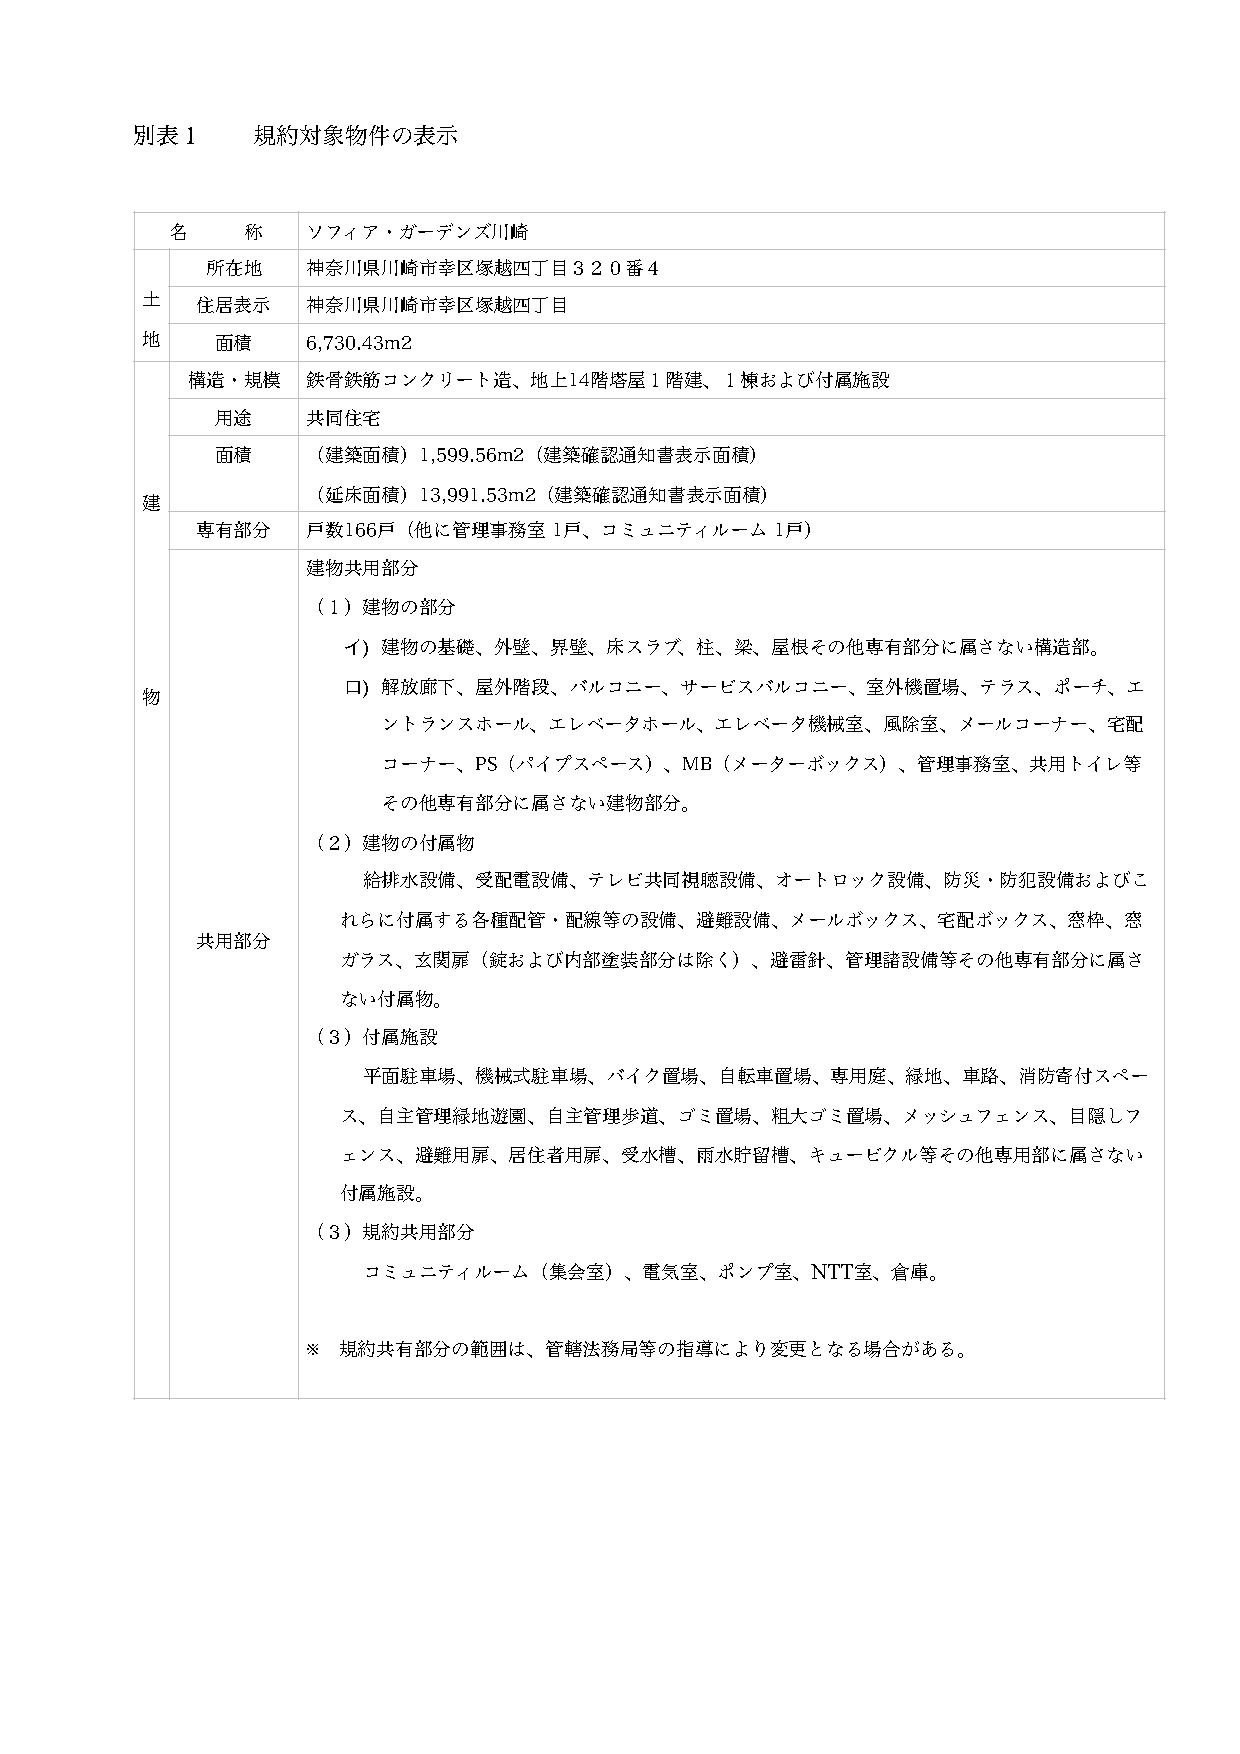
\includegraphics[scale=0.85]{table-1.pdf}
% \end{figure}
% 
% \begin{figure}[tp]
%   \addcontentsline{toc}{subsubsection}{別表2  土地および共用部分等における使用・専用使用に関する事項}
%   \addcontentsline{toc}{subsubsection}{別表3  機械式駐車場収容可能収容可能車}
%   \centering
%   \includegraphics[scale=0.85]{table-2.pdf}
% \end{figure}
% 
\end{document}